\subsection{RDF Vocabulary}

A mechanism for decentralized description and discovery of data was proposed
over two decades ago \textcolor{red}{cite https://www.w3.org/Talks/WWW94Tim/} 
and exists now in the tools and technologies of the Semantic Web. The 
specification of RDF as a data interchange format for the World Wide 
Web. \textcolor{red}{cite https://www.w3.org/RDF/?} is particularly relevant 
to our identified requirements. Decoupling publication 
from access meets many of these requirements (1, 4 and 5) and 
using RDF to describe log data collections provides decentralization 
and discovery without requiring a priori knowledge of other collection 
efforts.

In RDF \emph{things} (concepts or concrete items) are represented as URIs
and arranged in \emph{triples} of a subject, a predicate and an object.  

\begin{figure*}
\begin{minted}{turtle}
@prefix nersc: <http://portal.nersc.gov/project/mpccc/sleak/nersc#> .
@prefix rdfs: <http://www.w3.org/2000/01/rdf-schema#> .
@prefix foaf: <http://xmlns.com/foaf/0.1/> .
nersc:nersc rdfs:type foaf:Organization .
\end{minted}

\caption{A triple of (subject, predicate, object) describes an edge 
in an RDF graph. The \texttt{Turtle}\textcolor{red}{cite} syntax shown
here aids human readability by condensing URIs into a prefix and a suffix,
so for example \texttt{rdfs:type} expands as
\texttt{<http://www.w3.org/2000/01/rdf-schema\#type>}.}
\label{f:rdftriples}
\end{figure*}

For example, we wish to state that NERSC is an Organization. We have a 
\emph{subject} (NERSC), a \emph{predicate} (``is an'') and an \emph{object} 
(Organization). In a manner of pulling oneself up by one's bootstraps, the 
W3C \textcolor{red}{cite https://www.w3.org/} publishes some standard 
vocabularies in the form of URIs that have a well-defined and documented 
meaning, including that \texttt{<http://www.w3.org/2000/01/rdf-schema\#type>}
refers to the predicate ``is a''. Another vocabulary, known as the 
Friend-of-a-friend vocabularies, associates \texttt{<http://xmlns.com/foaf/0.1/Organization>} with the concept of an 
organization. In this spirit we write the triple in Figure~\ref{f:rdftriples}
by associating a URI we've chosen: \texttt{<http://portal.nersc.gov/project/mpccc/sleak/nersc\#nersc>} with the 
organization we know as ``NERSC''. 

A single triple tells us very little, but a collection of many triples 
forms a graph representing almost arbitrary knowledge graph. We get 
decentralization by the use of URIs as graph elements - any contributer 
can publish a set of triples and, so long as \emph{somebody} is aware of 
it, it can be incorporated into a global graph.

The other Semantic Web element key to our requirements is the SPARQL 
graph query language. A SPARQL query 
arranges variables into a set of triples and returns nodes for which
the triples form a true statement. For example, the following SPARQL query
will return the name and interest for each node whose type is 
a subclass of \texttt{foaf:Agent}. \texttt{foaf:Agent} is a superclass for a Person, a 
Group or an Organization, so this query in English is ``list the name and 
interest for each Person, Group or Organization in this graph''. (The 
\texttt{rdfs:subClassOf*} syntax indicates that the query should follow 
\texttt{rdfs:subClassOf} edges to any depth until a \texttt{foaf:Agent} 
is encountered).

\begin{figure}[H]
\begin{minted}{sparql}
SELECT ?name ?interest 
WHERE {    
    ?type rdfs:subClassOf* foaf:Agent .
    ?uri rdfs:type ?type .
    ?uri foaf:name ?name .
    ?uri foaf:interest ?interest .
}
\end{minted}
\caption{Example of a SPARQL query}
\label{f:sparql}
\end{figure}

Figure~\ref{f:sparql-diagram} illustrates how this query might act on a graph: 
the first statement locates nodes - colored blue - from which one can traverse \texttt{rdfs:subClassOf} edges and reach a \texttt{foaf:Agent}. The second statement 
locates nodes (shown in red) in triples with an \texttt{rdfs:type} predicate whose object 
is one found by the first statement. Thus far we have found Jim, 
Ann, Annette and Steve. Next we look for triples whose subject is one of those nodes
and whose predicate is \texttt{foaf:name}, reducing the set to Jim, Ann and Steve, then
again for predicate \texttt{foaf:interest}. Now only Steve matches all of the criteria.
Finally, we return the nodes associated with the \texttt{name} and \texttt{interest} 
variables, which in this case are the nodes show in purple.

\begin{figure}
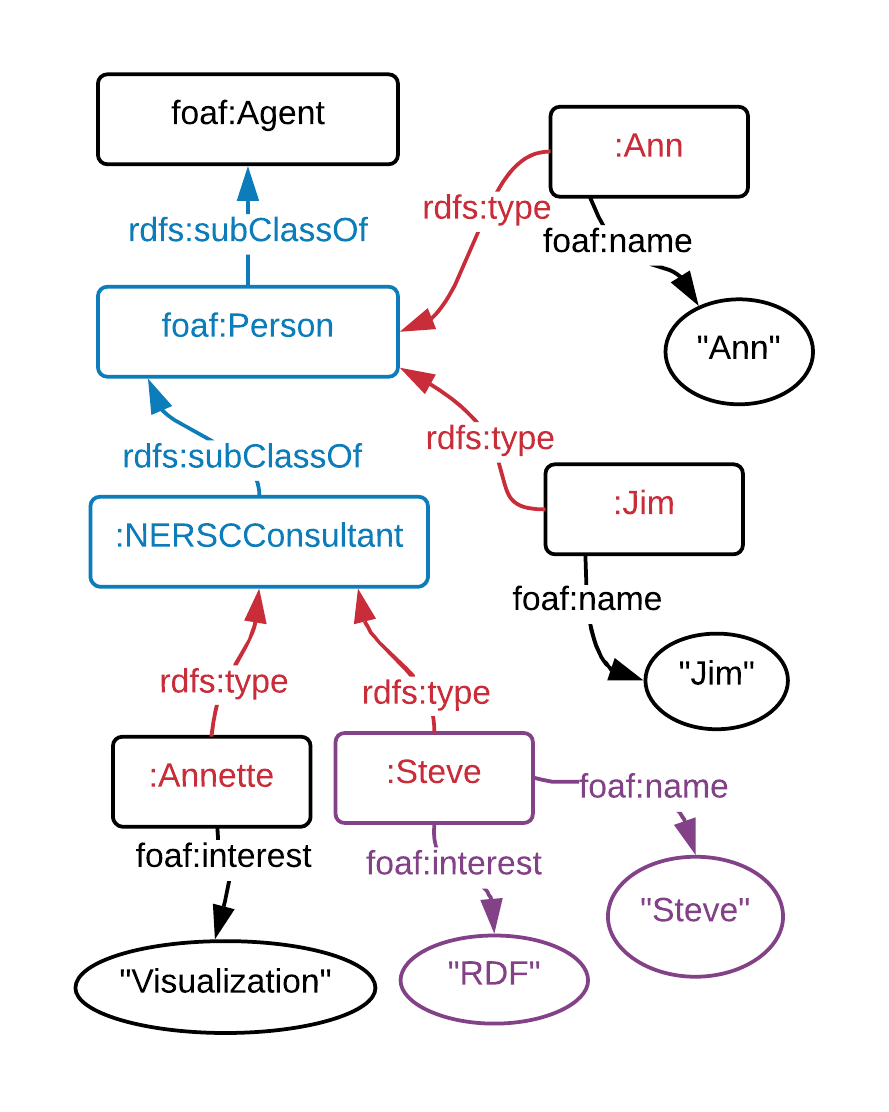
\includegraphics[width=0.4\textwidth]{sparql.png}
\caption{Illustration of the SPARQL query in Figure~\ref{f:sparql} }
\label{f:sparql-diagram}
\end{figure}

\textcolor{red}{TODO: might need a ref to an "intro to semantic web" resource}


\subsubsection{The vocabulary}

\begin{figure*}
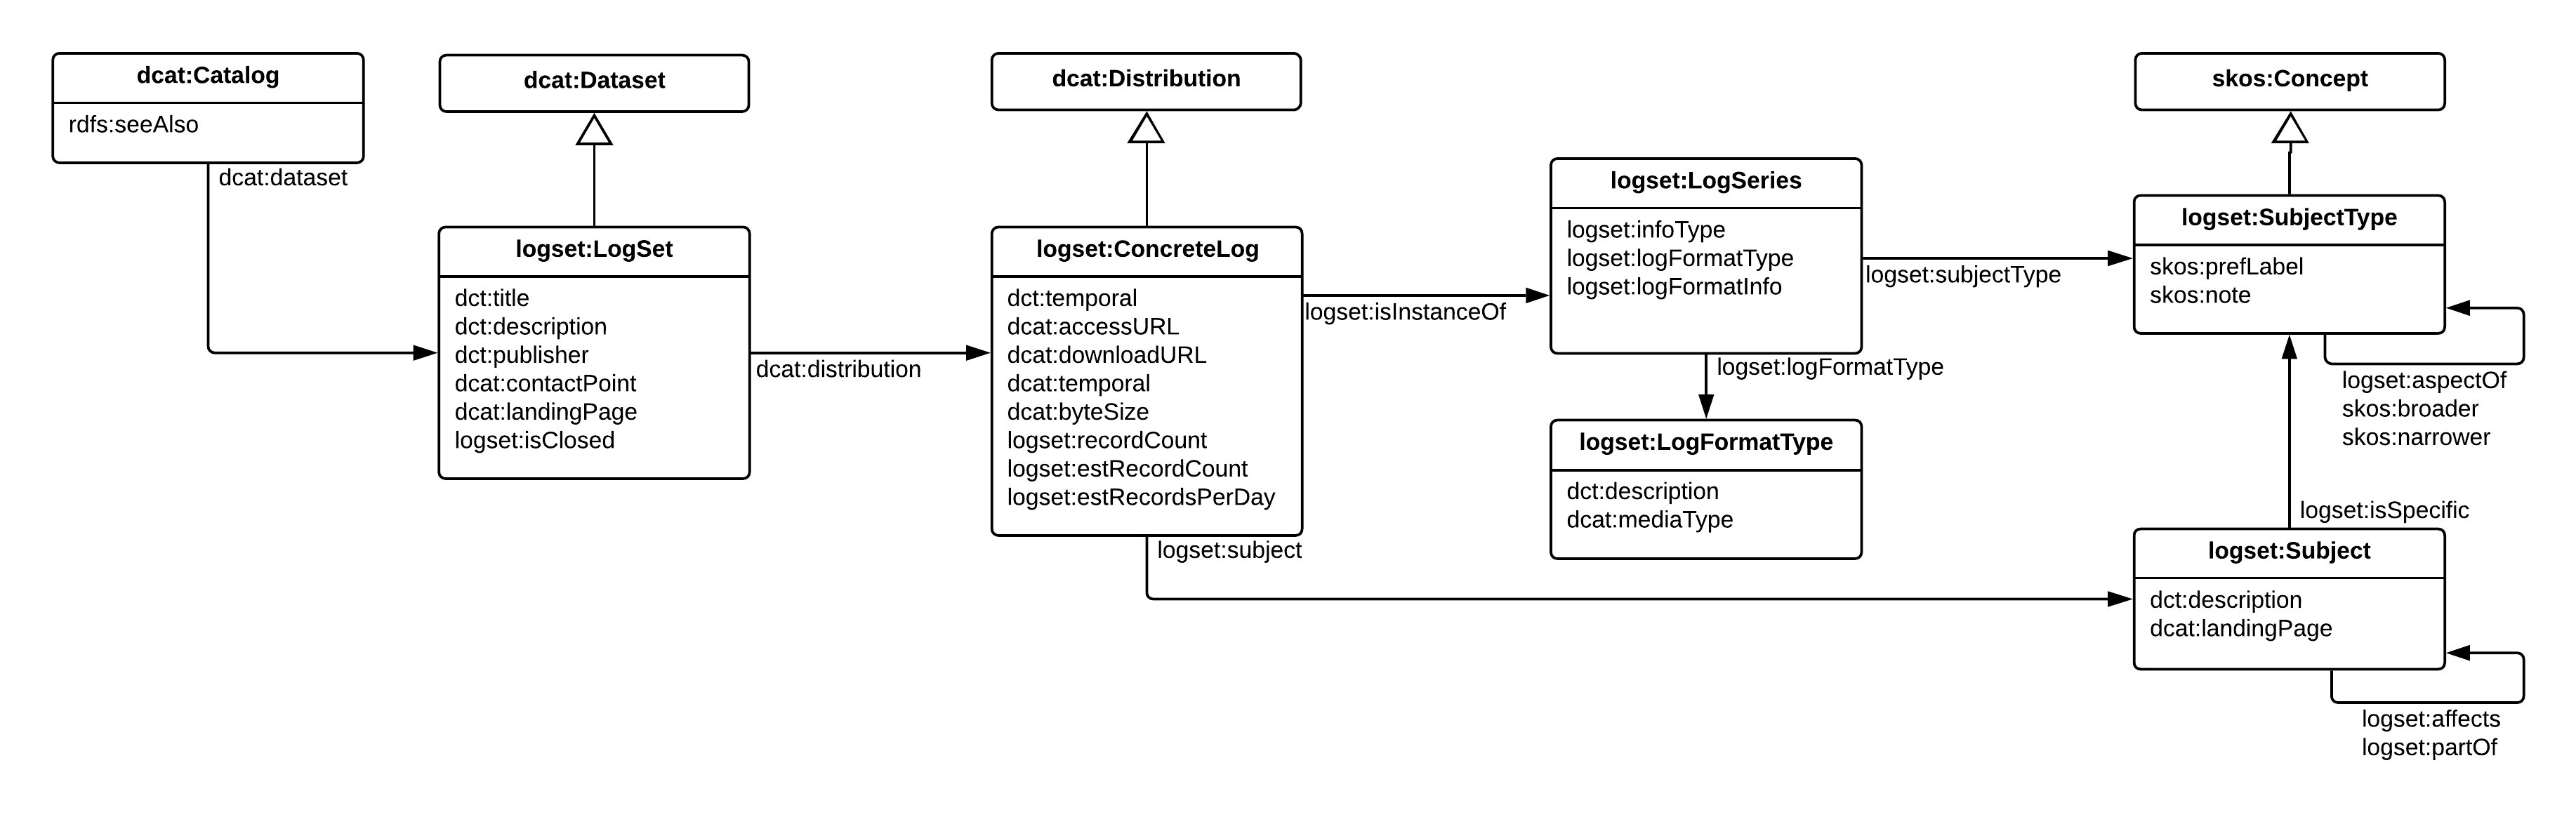
\includegraphics[width=1.0\textwidth]{logset-key-classes.png}
\caption{Key classes and predicates in the logset vocabulary. }
\label{f:logset-classes}
\end{figure*}

The key classes and predicates forming our vocabulary are illustrated in 
Figure~\ref{f:logset-classes}. Figure~\ref{f:logset-classes-nodes} provides 
examples of nodes in a graph corresponding to each class, and 
Figure~\ref{f:logset-example} shows how RDF descriptions of different
\texttt{LogSet}s published in different places form a single, global graph.
Figure~\ref{f:logset-example} also shows how data dictionaries 
describing different \texttt{SubjectType}s and \texttt{LogSeries} can be 
published and become part of the global graph when used.


\begin{figure*}
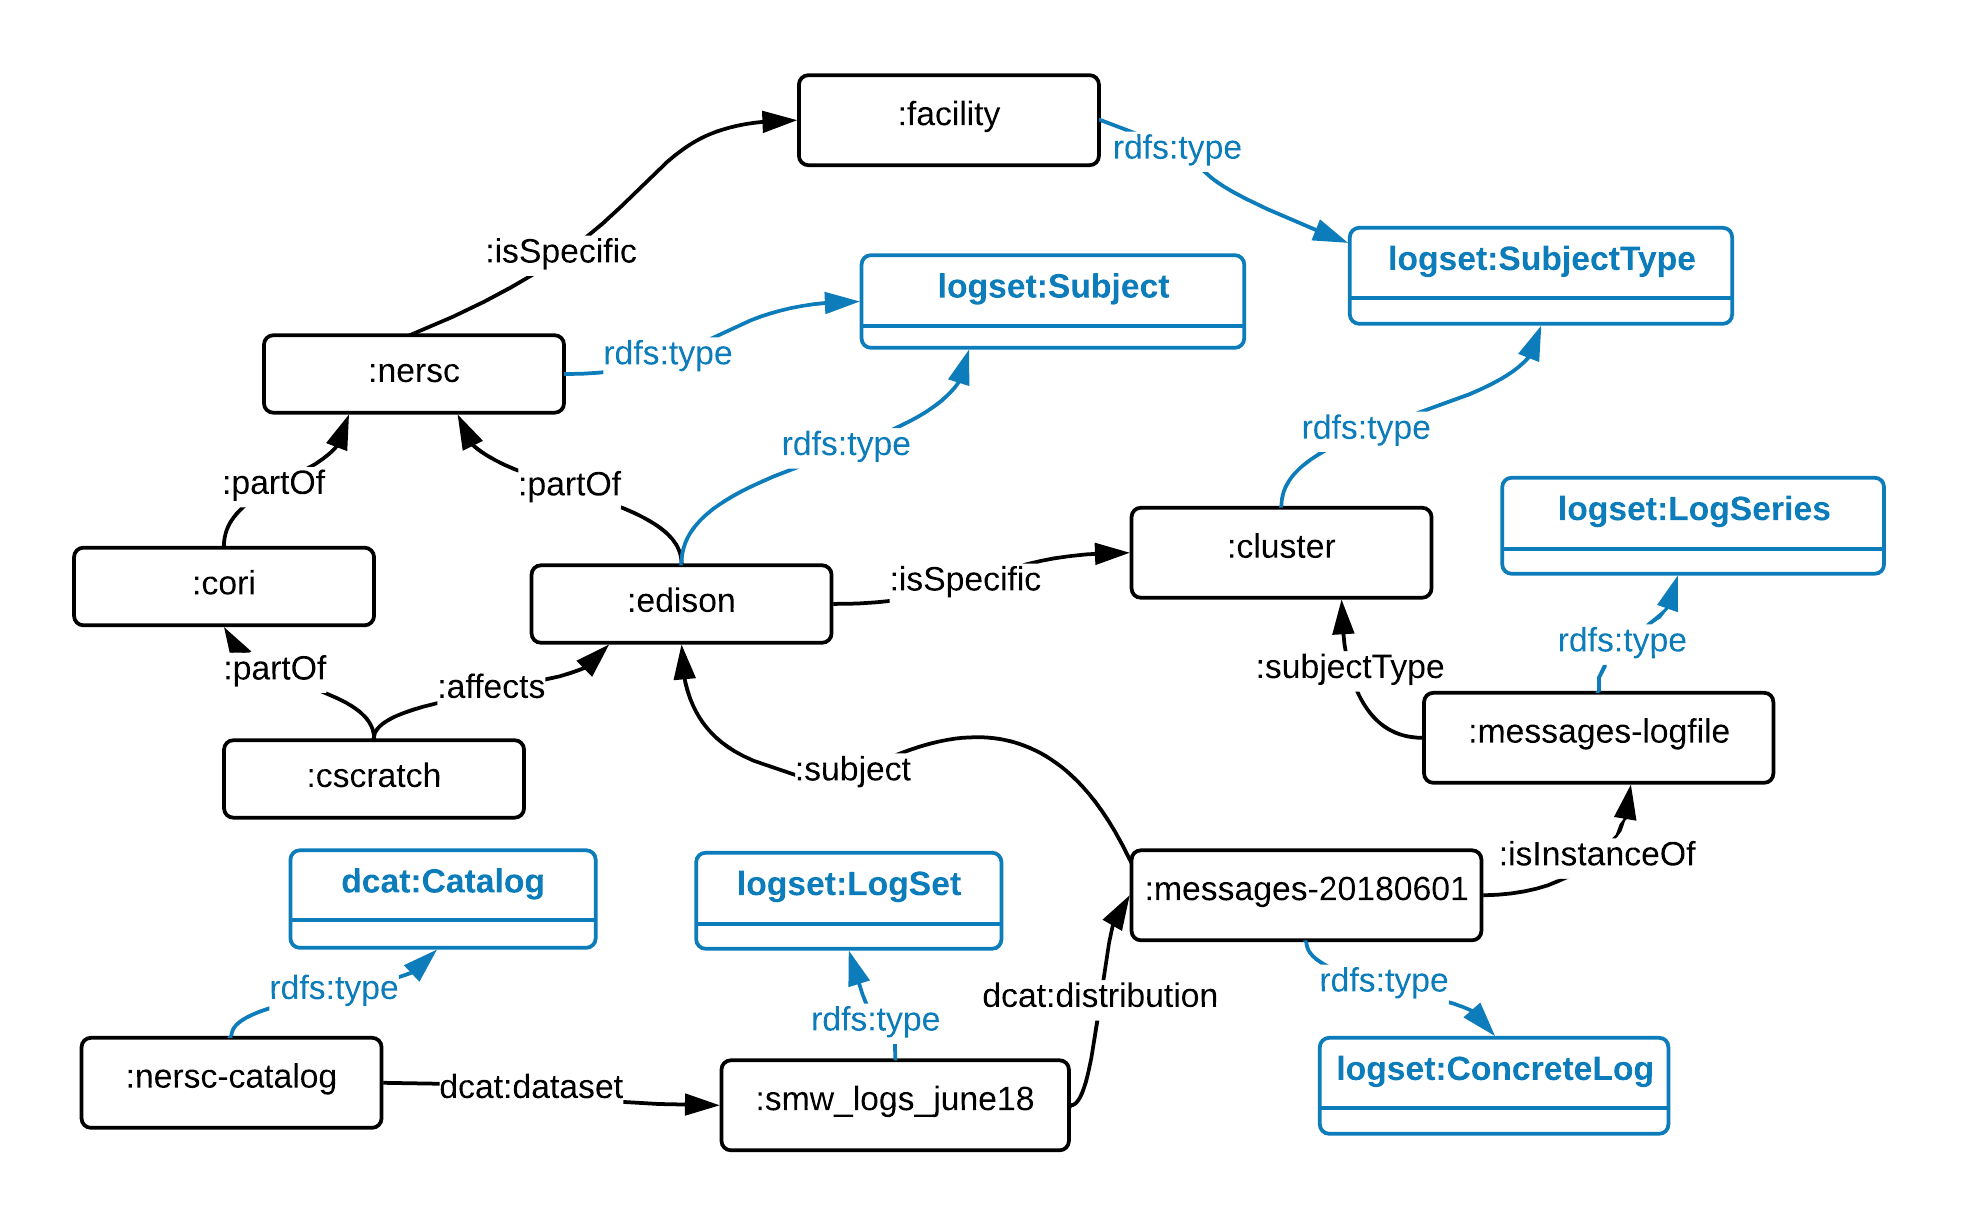
\includegraphics[width=0.9\textwidth]{logset-classes-nodes.png}
\caption{Examples of nodes in the graph and how they relate to
vocabulary classes}
\label{f:logset-classes-nodes}
\end{figure*}

\begin{figure*}
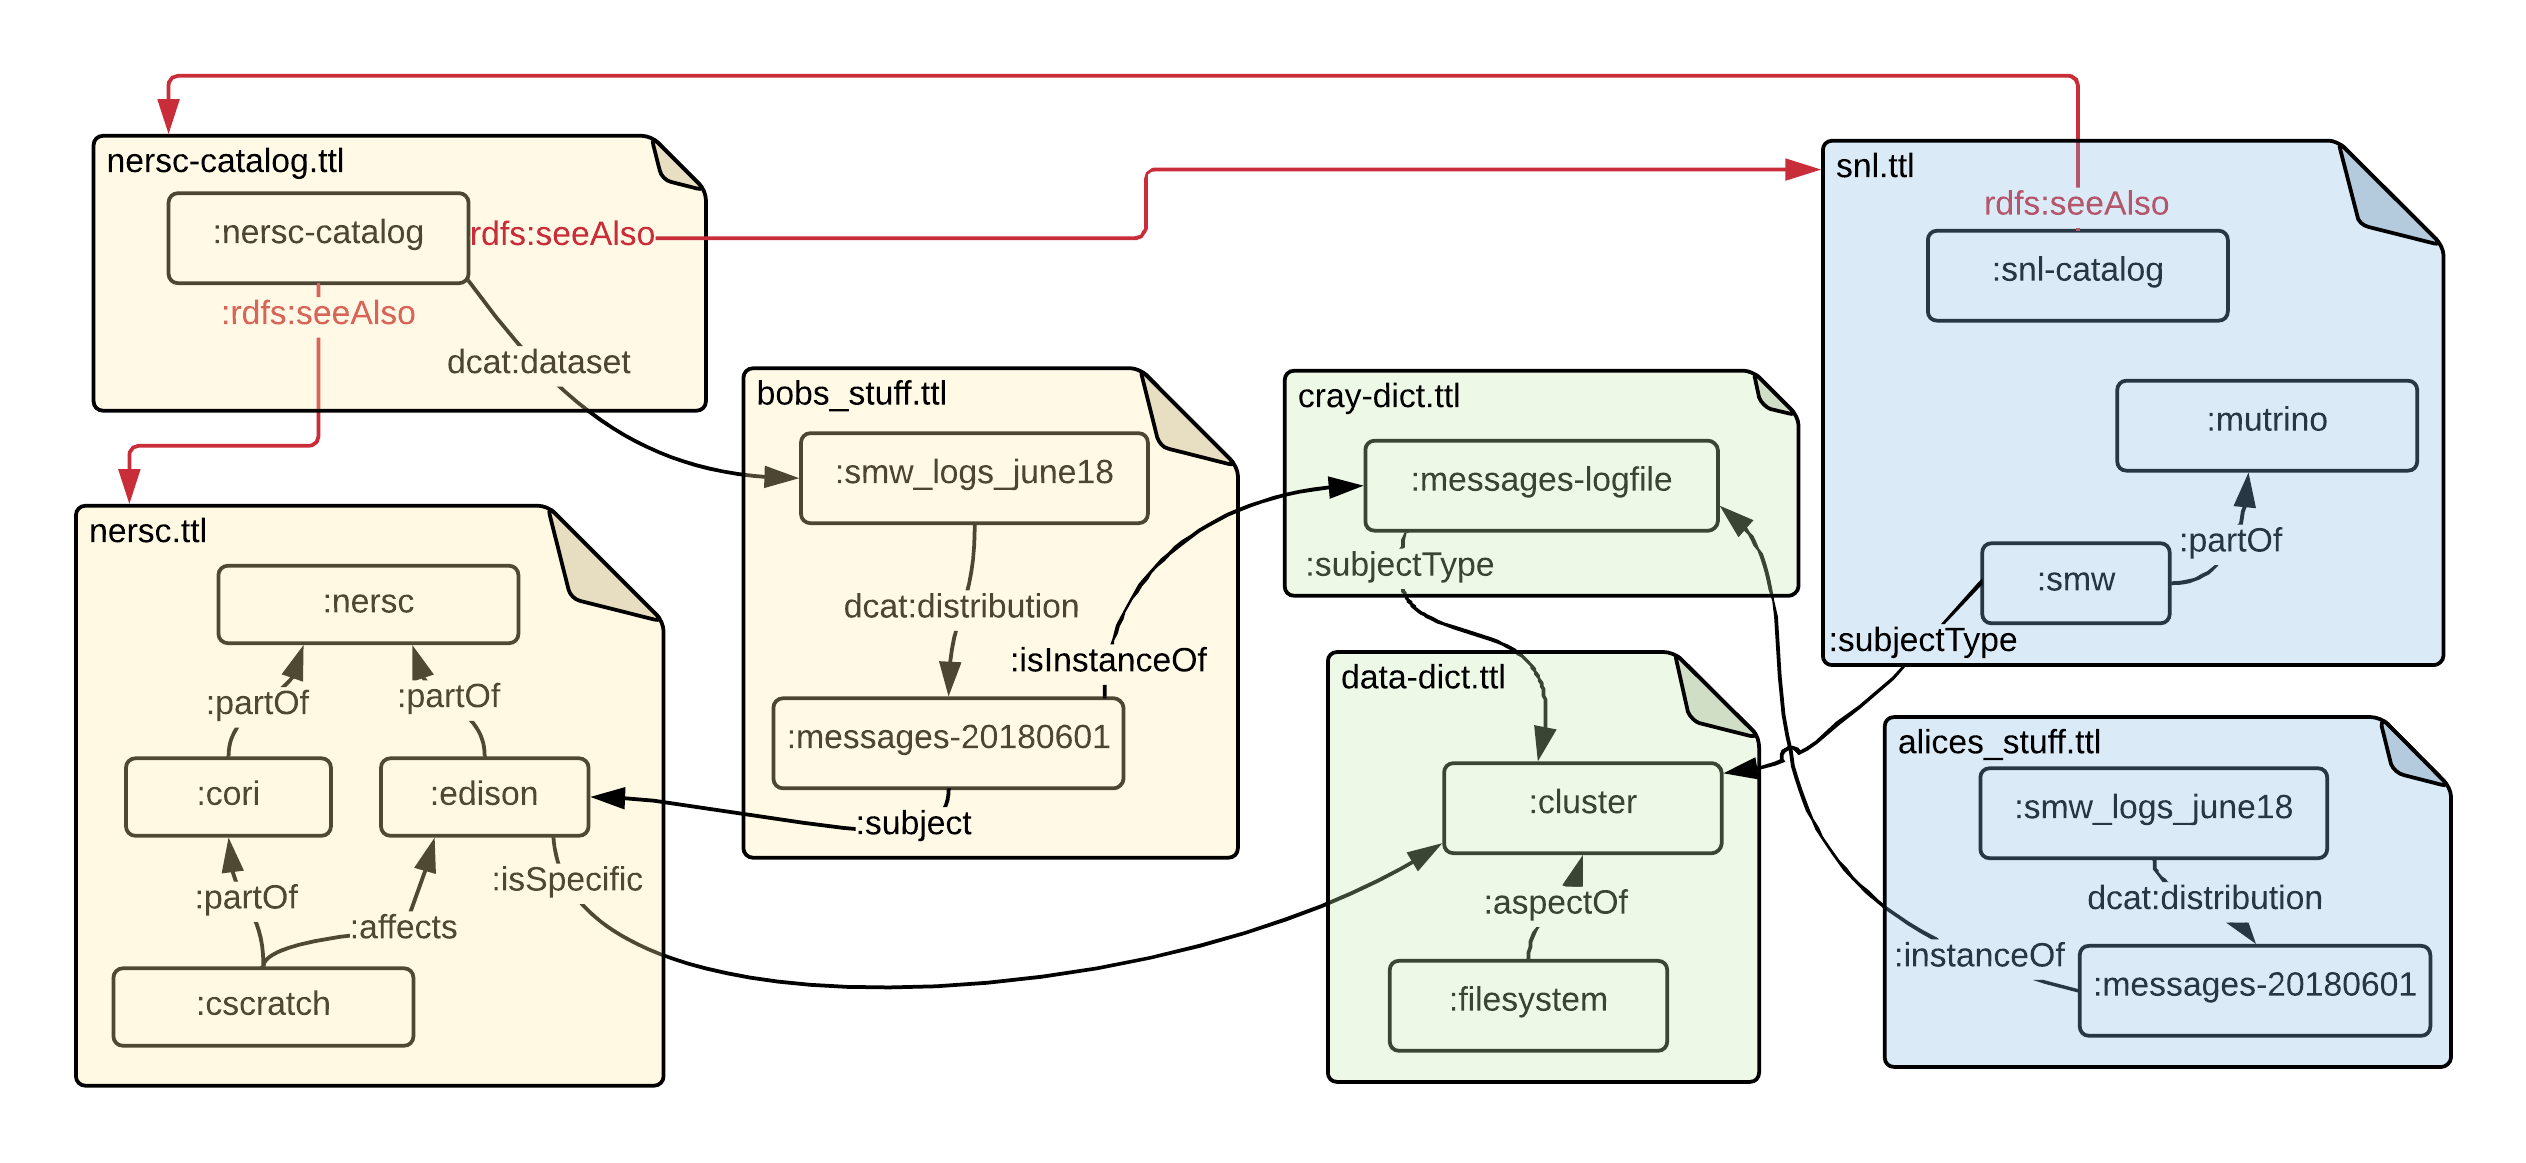
\includegraphics[width=0.9\textwidth]{logset-example.png}
\caption{Examples of some nodes and relationships published in different places 
from different sites (indicated via color), forming a single global graph. }
\label{f:logset-example}
\end{figure*}

The vocabulary is extended and specialized 
from the Data Catalog Vocabulary \textcolor{red}{cite}. The meaning, 
reason and usage of some key classes and properties:

\begin{description}
\item[Catalog] \hfill

The \texttt{dcat:Catalog} class connects \texttt{LogSet}s and also, via 
\texttt{rdfs:seeAlso}, other catalogs. This is the primary mechanism for 
linking sites into a global graph: we anticipate that each site will 
publish a catalog to which its own staff can contribute \texttt{LogSet}s, and which is linked to a few other sites via \texttt{rdfs:seeAlso}.

\item[LogSet] \hfill

A collection of logs related in system and access and timespan,
for example the logs collected in a \texttt{p0-} directory in the SMW of a Cray
XC for a single boot session. The \texttt{LogSet} should provide a description
of the data and contact information and is an entry point to metadata for 
the \texttt{ConcreteLog}s. Temporal and subject information for the \texttt{LogSet}
can be infered from those properties of its \texttt{ConcreteLog}s.

A \texttt{LogSet} might be a closed archive or might be ``open'',
acquiring new logs over time. 

\item[ConcreteLog] \hfill

A \texttt{ConcreteLog} describes a specific, concrete source of log entries.
This will often be a log file but could also be, for example, a Slurm instance
from which job data can be obtained. 

The \texttt{accessURL} and \texttt{downloadURL} have subtly different uses,
inherited from \texttt{dcat:Distribution}. Where security or practical 
constraints preclude direct download of data, \texttt{accessURL} can be used 
instead to find more information (such as how to request access).

The \texttt{ConcreteLog} should also include the 
start and (optional) end dates encompassed by the log. Inclusion of 
information about the size and number of records is also recommended, as a
means of avoiding download of excessively large data volumes.

\item[LogSeries] \hfill

Most log data can be classified into a few \emph{series}, such as 
``console log files'' or ``Slurm job records''. \texttt{ConcreteLog}s
within a \texttt{LogSeries} have the same structure but span different 
times or subjects. A \texttt{LogSeries} is often common to systems from a
given vendor and is expected to be published in a common dictionary.

\item[LogFormatType] \hfill

The \texttt{LogFormatType} gives hints to tools about how a particular
\texttt{LogSeries} should be handled. For example, many logs are in the
form of a \texttt{timeStampedLogFile}. Series-specific details such 
as how to identify the timestamp of a record is published in the 
\texttt{logFormatInfo} property of the \texttt{LogSeries}.
 
\item[Subject] \hfill

Logs are about \emph{something} - e.g. the cluster, a specific service
node or the filesystem, so each \texttt{ConcreteLog} should indicate
this. Subjects mostly correspond to Cluster components, and can be 
assembled into a hierarchy via a \texttt{partOf} property. Not all 
relationships are hierarchical - for example a network link impacts
the device on each end - so we support a weaker relationship 
\texttt{affects} as well.

\item[SubjectType] \hfill

In the same way that \texttt{ConcreteLog}s can be classified into 
\texttt{LogSeries}, \texttt{Subject}s can be classified into 
\texttt{SubjectType}s. An example \texttt{SubjectType} is ``cluster'',
compared to an example \texttt{Subject}, NERSC Cori. During the
procedure of cataloging LogSets, the graph can be queried to see that
a specific \texttt{LogSeries} is about a \texttt{SubjectType} 
\texttt{hsn}, from which tools can infer that a specific 
\texttt{ConcreteLog} should be associated with \texttt{cori\_hsn}.
(This inference capability is essential when cataloging thousands of 
log files)

\texttt{SubjectType} based on the \texttt{skos:Concept}, through 
which \texttt{SubjectType}s can be classified as broader or narrower
that each other (``network'' is a broader concept than ``AriesHSN'').

\end{description}






